\documentclass{scrartcl}
\usepackage{etoolbox}
\usepackage{bbm}
\usepackage{amsmath}
\usepackage{mathabx}
\usepackage{graphicx}
\usepackage{float}
\usepackage{parskip}
\usepackage{indentfirst}
\usepackage{subfig}
\usepackage{fancyhdr}
\usepackage{hyperref}
\pagestyle{fancy}
\setlength{\parskip}{0em}
\setlength{\parindent}{2em}

%-----------------------------------------------------------------------------
\begin{document}

%-----------------------------------------------------------------------------
% header
\lhead{Huwenbo Shi (603-778-363) shihuwenbo@ucla.edu}

% title
\newcommand*{\TitleFont}{
      \usefont{\encodingdefault}{\rmdefault}{b}{n}
      \fontsize{16}{20}
      \selectfont}
\newcommand*{\AuthorFont}{
      \usefont{\encodingdefault}{\rmdefault}{r}{n}
      \fontsize{12}{20}
      \selectfont}
\title{\TitleFont SoCal: supervised genotype calling via ellipsoid
separation for Affymetrix SNP microarray}
\author{\AuthorFont Huwenbo Shi (603-778-363) shihuwenbo@ucla.edu}
\date{}
\maketitle
%-----------------------------------------------------------------------------





%-----------------------------------------------------------------------------
% abstract
\begin{abstract}

\centerline{ABSTRACT}

\vspace*{\baselineskip}

\par
In this article, I present SoCal, a supervised genotype calling algorithm for
Affymetrix SNP microarray.
For each SNP, SoCal first efficiently identify ellipsoidal decision regions for
each genotype from reference genotype calls, and then uses these regions to
classify future SNPs into different genotypes.
Using only a small portion of training genotype calls from the HapMap Project,
SoCal achieves an accuracy of $97.5\%$ during validation.

\end{abstract}
%-----------------------------------------------------------------------------





%-----------------------------------------------------------------------------
% introduction
\section{Introduction}

\par
% broad background
Accurate genotyping of SNPs is essential to discovering true signals in
association studies.
Although next generation sequencing technology provides cheap whole-genome
sequences for genotyping SNPs, SNP microarray is still a cost-effective
genotyping technology for many specific association studies.
In an Affymetrix SNP microarray, oligonucleotide probes are used to match and
bind DNA fragments containing biallelic SNPs.
Then a fluorescence scanner scans the microarray to quantify perfect 
match and mismatch of these fragments.
Most genotype calling procedures for SNP microarray consists of two steps.
In the first step, raw information from microarray is summarized to obtain the
intensities, $\theta_A$ and $\theta_B$, of the two alleles, denoted by A and B,
of each SNP.
In the second step, SNPs are classified into genotype AA, AB, or BB based on
the allele intensities they generate.
The focus of this article is on the second step of the genotype calling
procedure---genotype calling using summarized allele intensities.

\par
% specific background
For a specific SNP, if a sample has genotype AA or BB, the allele intensity,
$\theta_A$ or $\theta_B$, will be higher respectively. 
If a sample has genotype AB, the intensities, $\theta_A$ and $\theta_B$,
will be similar.
If one plots $log(\theta_A)$ versus $log(\theta_B)$ of a SNP for a number of
samples, normally 3 ellipsoidal clusters can be observed, one for each
genotype, as shown in Figure~\ref{fig:intro_genclus}.
% state the problem
Many genotype calling algorithms use model-based unsupervised clustering
to identify these clusters and then assign genotypes to each cluster.
Although these methods are applicable to a wide range of microarrays, they
don't take advantage of genotype calls that are already available.
Also, these methods use the EM algorithm to estimate model parameters, which is
sensitive to starting parameters and slow to converge.
To utilize reference genotype calls, Rabbee et al. proposed the RLMM algorithm,
a supervised genotype calling method that uses reference genotype calls to form
decision regions by fitting bivariate Gaussian distributions on observed
allele intensities for each genotype.
These Gaussian decision regions are then used to call SNPs with unknown
genotype.
However, fitting a Gaussian distribution is known to be sensitive to outliers,
which, for SNP microarrays, can be caused by genomic structural variations.

% intro genotype cluster figure
\begin{figure}[H]
\centering
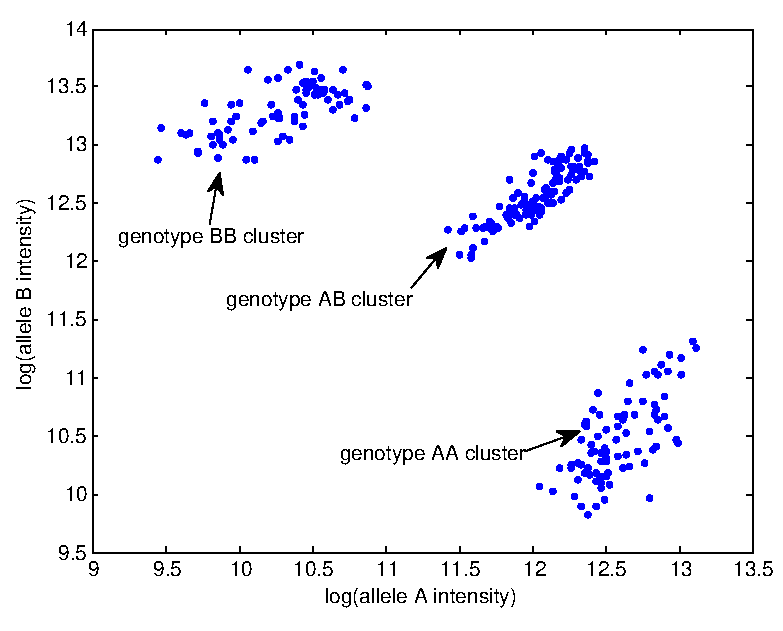
\includegraphics[scale=0.75]{intro_figs/intro_genotype_clusters.pdf}
\caption{Genotype clusters obtained from Affymetrix SNP array
allele intensity values}
\label{fig:intro_genclus}
\end{figure}

\par
% state my solution
In this article, I present SoCal, a supervised genotype calling algorithm
for Affymetrix SNP microarrays.
Instead of fitting Gaussian distributions on allele intensities with reference
genotype calls, SoCal efficiently finds ellipsoidal decision regions for each
genotype of a SNP by solving a conic programming problem.
SoCal can control the effect of outliers by assigning different weights to each
of the criteria for finding the ellipsoids---separation ratio, ellipsoid
volume, and number of enclosed points. 
After SoCal finds the ellipsoidal decision regions for each genotype of
a SNP, it uses them to call the same SNP with unknown genotype.

\par
% state the result
Using reference genotype calls from the HapMap Project as training and
validation data, SoCal achieved $99.71\%$ accuracy at a call rate of $95\%$
during leave-one-out cross-validation.
Furthermore, SoCal shows more robustness than the RLMM method when there are
outliers in the training data.
%-----------------------------------------------------------------------------





%-----------------------------------------------------------------------------
% method
\section{Methods}

% overview of method
\subsection{Overview of SoCal's genotype calling procedure}

\par
SNP allele intensities are first summarized from raw microarray data using
SNPRMA, which removes non-biological effect from the data.
After this step, SoCal calls genotypes in two steps.
In the first step, SoCal finds ellipsoidal decision regions for each of the
genotype of a SNP using reference genotype calls.
In the second step, SoCal classifies SNPs with unknown genotypes using
minimum distance classification.

% pattern separation via ellipsoids
\subsection{Pattern separation by ellipsoid}

\par
An ellipsoid $\mathcal{E} \subseteq \mathbbm{R}^{n}$ can be expressed as
$\mathcal{E} = \{x \in \mathbbm{R}^{n} | (x-c)^TE(x-c)\leqslant1\}$, where
$c$ is the center of the ellipsoid, and $E$ a positive definite matrix
denoting the shape and orientation of the ellipsoid.
Let $\{a_i\}$ be the points to be included in an ellipsoid, and $\{b_j\}$
be the points to be excluded, the problem of ellipsoidal separation is to find
$c$ and $E$ such that $(a_i-c)^TE(a_i-c)\leqslant1 \, \forall i$ and
$(b_j-c)^TE(b_j-c)>1 \, \forall j$.

% ellipsoidal pattern separation formulation
\subsection{Forming ellipsoidal decision regions for each genotype}

\par
Let $G=\{AA,AB,BB\}$ be the set of genotypes of a SNP, and $J_{AA}$, $J_{AB}$,
$J_{BB}$ the index set of samples with the corresponding genotype.
Let $X=\{(log(\theta_A),log(\theta_B))_i|i=1,\cdots,
|J_{AA}|+|J_{AB}|+|J_{BB}|\}$ be the set of log transformed allele intensities
of all the samples, and $X_{AA}=\{x_j|x_j \in X, j \in J_{AA}\}$,
$X_{AB}=\{x_j|x_j \in X, j \in J_{AB}\}$,
$X_{BB}=\{x_j|x_j \in X, j \in J_{BB}\}$ the set of log transformed allele
intensities from samples having the corresponding genotype.

\par
To find the ellipsoid that includes $X_{AA}$ and excludes
$X_{AB} \cup X_{BB}$, one
sets $\{a_i\}=X_{AA}$ and $\{b_j\}=X_{AB} \cup X_{BB}$, and
solves the following conic programming problem.
The derivation of the problem formulation is largely followed from
\cite{glineur1998}.
For the sake of space, detailed derivation of the problem formulation is not
presented here.
\begin{equation*}
\begin{aligned}
& \text{minimize}
&& -{\beta_{1}}k+{\beta_{2}} trace(T)+\beta_{3} \|u-\mathbbm{1}\|_1 \\  
& \text{subject to}
&& (1,a_i)^T\tilde{E}(1,a_i)\leqslant u_i \; \forall i \\
&&&(1,b_j)^T\tilde{E}(1,b_j) \ge k \; \forall j \\
&&&\tilde{E}=
    \left[
        \begin{array}{cc}
            s & v^T \\
            v & F
        \end{array}
    \right] \succeq 0 \\
&&&\left[
        \begin{array}{cc}
            F & I \\
            I & T
        \end{array}
    \right] \succeq 0
\end{aligned}
\end{equation*}

\par
In the problem formulation above $\beta_{i} > 0$ are the weights assigned to
each criteria of finding the ellipsoid---separation ratio, ellipsoid volume,
and number of enclosed points.
In SoCal, $\beta_1$, $\beta_2$, $\beta_3$ are empirically set to 1, $10^4$,
and $10^2$ respectively.

\par
Let 
$\tilde{E}^{*}=\left[
    \begin{array}{cc}
    s & v^T \\
    v & F
    \end{array}
\right]$
be the optimal solution to the problem above.
The separating ellipsoid $\mathcal{E}^{*}$ is defined as
$\mathcal{E}^{*}=
\{x \in \mathbbm{R}^{n}|(x-c^{*})^TE^{*}(x-c^{*})\leqslant2(1+k)\}$,
where $c^{*}=-F^{-1}v,\;E^{*}={{F} \over {(1-s+{c^{*}}^TF{c^{*}})}}$.

\par
To find the ellipsoid that includes $X_{AB}$ and excludes
$X_{AA} \cup X_{BB}$, one sets $\{a_i\}=X_{AB}$ and
$\{b_j\}=X_{AA} \cup X_{BB}$, and solves the above conic programming problem.
The same procedure also applies to finding the ellipsoid that includes $X_{BB}$
and excludes $X_{AA} \cup X_{AB}$.
% handling missing clusters
\subsection{Rescuing missing genotype clusters}
\par
If a SNP has moderate minor allele frequency (MAF), the genotype clusters of
that SNP are well defined, and SoCal obtains three ellipsoidal decision
regions for that SNP, one for each genotype (Figure \ref{fig:defined_cluster}).
However, if a SNP has lower MAF, some genotype cluster may not be well defined.
For these SNPs, SoCal estimates the ellipsoid for the missing genotype cluster
using the ellipsoids for the other two genotypes through simple geometric
transformations (Figure \ref{fig:sparse_cluster}).

\begin{figure}[H]
    \centering
    \subfloat[SNP with well defined genotype clusters] {
        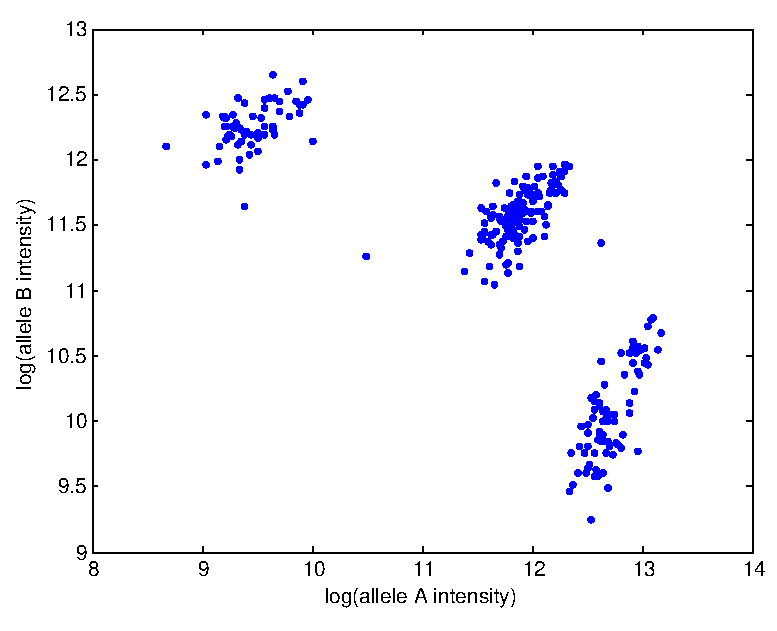
\includegraphics[scale=0.5]{method_figs/defined_cluster.pdf}
        \label{fig:defined_cluster}
    }
    \subfloat[SNP with sparse BB genotype cluster] {
        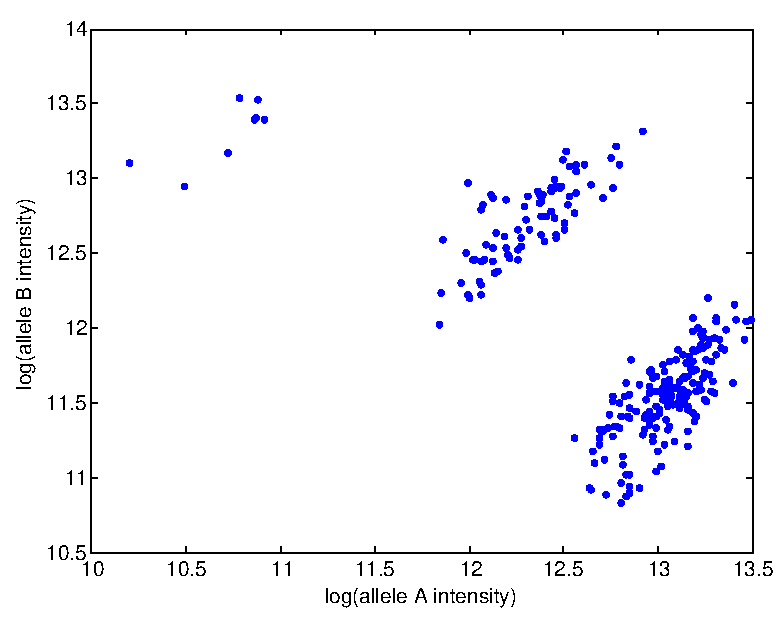
\includegraphics[scale=0.5]{method_figs/sparse_cluster.pdf}
        \label{fig:sparse_cluster}
    }
    \caption{Each dot in the plots above represents a sample, with
             samples having HapMap reference genotype calls marked red.
             The ellipsoids were obtained using only the reference calls.}
    \label{fig:defined_sparse_cluster}
\end{figure}

% missing genotype aa cluster
\subsubsection{Missing genotype AA or BB cluster}

\par
If genotype $AA$ cluster of a SNP has less than 3 reference calls, SoCal
first finds the ellipsoids for genotype $AB$ and $BB$ clusters, and then
estimates that for genotype $AA$ cluster through simple geometric
transformations.

\par
Let $\mathcal{E}_{AB}=
\{x \in \mathbbm{R}^{n}|(x-c_{AB})^TE_{AB}(x-c_{AB}) \leqslant 1\}$
and $\mathcal{E}_{BB}=
\{x \in \mathbbm{R}^{n}|(x-c_{BB})^TE_{BB}(x-c_{BB}) \leqslant 1\}$
be the ellipsoids obtained for genotype $AB$ and $BB$ clusters,
and $n_{AB}$, $n_{BB}$ the unit vectors pointing in the direction of
the major axis of the corresponding ellipsoid.
SoCal estimates the center of $\mathcal{E}_{AA}$, the ellipsoid for genotype
$AA$ cluster, by reflecting $c_{BB}$, the center of $\mathcal{E}_{BB}$, across
the major axis of $\mathcal{E}_{AB}$.
To estimate the orientation of $\mathcal{E}_{AA}$, SoCal first determines the
angle between $n_{AB}$ and $n_{BB}$, and then applies a rotation matrix of
that angle on $E_{AB}$.

\par
Formally, let $\mathcal{E}_{AA}=
\{x \in \mathbbm{R}^{n}|(x-c_{AA})^TE_{AA}(x-c_{AA}) \leqslant 1\}$ be the
estimated ellipsoid for genotype $AA$ cluster, and $\alpha$ the angle between
$n_{AB}$ and $n_{BB}$, then
$c_{AA}=-c_{BB}+2c_{AB}+2n_{AB}((c_{BB}-c_{AB})^{T}n_{AB})$, and
$E_{AA}=R^{T}E_{AB}R$, where $R$ is a rotation matrix of angle $\alpha$.

\par
If genotype $BB$ cluster is missing, the center and orientation of the
ellipsoid for that cluster is estimated in a similar way.
Formally, let $\mathcal{E}_{BB}=
\{x \in \mathbbm{R}^{n}|(x-c_{BB})^TE_{BB}(x-c_{BB}) \leqslant 1\}$ be the
estimated ellipsoid for genotype $BB$ cluster, and $\alpha$ the angle between
$n_{AB}$ and $n_{AA}$, then
$c_{BB}=-c_{AA}+2c_{AB}+2n_{AB}((c_{AA}-c_{AB})^{T}n_{AB})$, and
$E_{BB}=R^{T}E_{AB}R$, where $R$ is a rotation matrix of angle $-\alpha$.

% missing genotype ab cluster
\subsubsection{Missing genotype AB cluster}

Although SNPs with genotype $AB$ cluster missing were not observed in HapMap
reference genotype calls, for completeness, for these SNPs SoCal first
obtains, $\mathcal{E}_{AA}$ and $\mathcal{E}_{BB}$,
the ellipsoids for genotype $AA$ and $BB$ cluster, and then estimates the
center of $\mathcal{E}_{AB}$, the ellipsoid for the missing cluster, using
the mid-point between the centers of $\mathcal{E}_{AA}$ and $\mathcal{E}_{BB}$.
The orientation of $\mathcal{E}_{AB}$ is obtained by applying a rotation
to the ellipsoid with the minimum volume among $\mathcal{E}_{AA}$ and
$\mathcal{E}_{BB}$.

\par
Formally, let $\mathcal{E}_{AB}=
\{x \in \mathbbm{R}^{n}|(x-c_{AB})^TE_{AB}(x-c_{AB}) \leqslant 1\}$ be the
estimated ellipsoid for genotype $AB$ cluster, and $\alpha$ the angle between
$n_{AA}$ and $n_{BB}$, then
$c_{AB}=(c_{AA}+c_{BB})/2$, and
$E_{AB}=R^{T}\hat{E}R$, where $\hat{E}$ is the matrix of the ellipsoid
with the minimum volumne among $\mathcal{E}_{AA}$ and $\mathcal{E}_{BB}$, and
$R$ a rotation matrix of angle $\pm\alpha/2$.
The sign of the angle of rotation is dependent on the choise of ellipsoid on
which rotation is applied---positive for $\mathcal{E}_{AA}$ and negative
for $\mathcal{E}_{BB}$.

% genotype calling and outlier detection
\subsection{Genotype calling}

\par
After the ellipsoidal decision regions,
$\mathcal{E}_{g}=
\{x \in \mathbbm{R}^{n} | (x-c_g)^TE_g(x-c_g) \leqslant 1\},
\forall g\in\{AA,AB,BB\}$ of a SNP are obtained, SoCal uses them to classify
SNPs with unknown genotypes using minimum distance classification.

\par
If a sample has allele intensity $\theta_A$ and $\theta_B$ at SNP $n$,
SoCal first computes
$D_g=\sqrt{(x-c_g)^TE_g(x-c_g)}$,
where $x=(log(\theta_A), log(\theta_B))$, for each $g\in\{AA,AB,BB\}$.
SoCal then calls the genotype, $\mathcal{G}$, of that sample at SNP $n$
as the genotype having the minimum $D_g$, that is,
$\mathcal{G}=\operatorname*{arg\,min}_{g\in \{AA,AB,BB\}}D_g$.

\par
SoCal defines $\lambda=1-D_{\mathcal{G}}/(D_{AA}+D_{AB}+D_{BB})$ to quantify
the confidence of each genotype call.
By increasing the threshold for $\lambda$, SoCal can achieve higher call
accuracy at the cost of decreasing call rate.
%-----------------------------------------------------------------------------





%-----------------------------------------------------------------------------
% data
\section{Materials}

\par
The microarray used for evaluation in this project was the Affymetrix GeneChip
Human Mapping 50K Xba Array, which contains 58,960 SNPs.
Raw microarray data for 270 samples was obtained from HapMap FTP.
And reference genotype calls were obtained from HapMap using HapMart.

\par
After removing strand-ambiguous SNPs and SNPs not present on HapMart from
the microarry, 16,387 SNPs were left.
Figure~\ref{fig:data_maf_dist} shows the minor allele frequency distribution
for these SNPs.

% maf distribution figure
\begin{figure}[H]
\centering
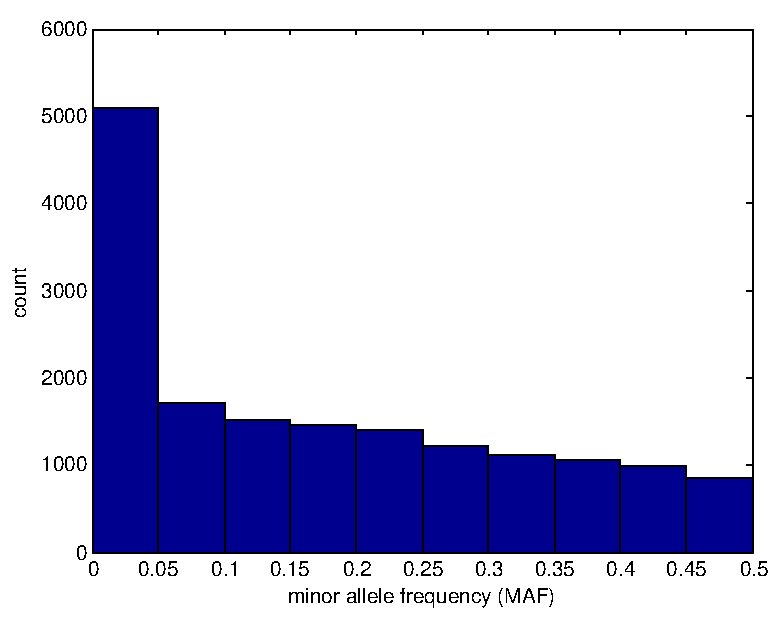
\includegraphics[scale=0.75]
{data_figs/maf_dist.pdf}
\caption{Minor allele frequency distribution for the 16,387 SNPs.}
\label{fig:data_maf_dist}
\end{figure}


\par
From the 16,387 SNPs, 4,064 SNPs with two genotype clusters having less than
3 reference genotype calls were further removed from the microarry.
Among these SNPs, 3,596 are monomorphic SNPs.
In total, 12,323 SNPs were left for evaluation.
On average, each of these SNPs has 83 reference genotype calls.
%-----------------------------------------------------------------------------





%-----------------------------------------------------------------------------
% result
\section{Results}

% result for comparing socal with hapmap calls
\subsection{Cross-validation with HapMap reference calls}

\par
To evaluate the accuracy of SoCal, I compared the genotype calls made by SoCal
with the reference calls from HapMap through leave-one-out
cross-validation.
For each SNP, I used one sample from the reference set as validation data and
the rest as training data.
I repeated this process until all the samples in the reference set were used
as validation data exactly once.

\par
First, I compared the accuracy of SoCal under different choices of $\beta_i$,
which are the weights assigned to the criteria of finding the ellipsoidal
decision regions for each genotype cluster.
Figure~\ref{fig:result_sh_crvacc} shows the concordance rate of SoCal in the
leave-one-out cross-validation for a wide range of call rates when different
values of $\beta_i$ were used.
Because the choice of weights, $\beta_1=1$, $\beta_2=10^4$, $\beta_3=10^2$,
had the highest call rate at fixed concordance rates, it's set to be the
default choice of SoCal.
And all future experiments presented in this article used this choice
of weights.

% accuracy as function of call rate
\begin{figure}[H]
\centering
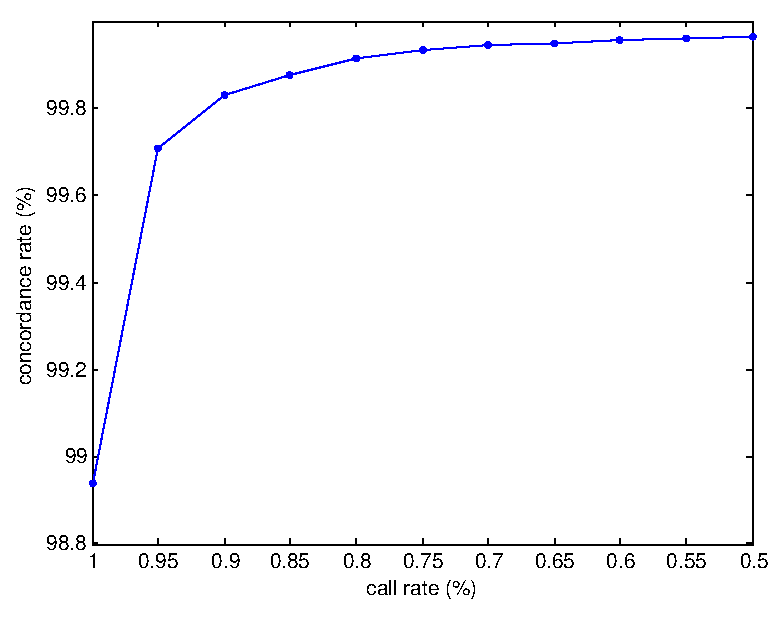
\includegraphics[scale=0.75]
{result_figs/cmp_socal_hapmap/cmp_socal_hapmap_cr_vs_acc.pdf}
\caption{Concordance rate of SoCal in the leave-one-out cross-validation with
HapMap reference calls as a function of call rate, for different choices of
$\beta_i$}
\label{fig:result_sh_crvacc}
\end{figure}

\par
Table~\ref{table:cmp_hapmap_socal_100} shows the genotype calls made by SoCal
and those available on HapMap during leave-one-out cross-validation.
At a call rate of 100\%, SoCal made 1,081,319 calls in total, out of which
1,069,857 were concordant with HapMap calls, achieving a concordance
rate of 98.94\%.

% 100% call rate result
\begin{table}[H]
\centering
\begin{tabular}{l*{5}{r}r}
    \hline
    HapMap/SoCal  & AA       & AB      & BB      & No Call \\ \hline
    AA            & 360,289  & 2,282   & 1,058   & 0  \\
    AB            & 2,667    & 341,012 & 2,257   & 0  \\
    BB            & 851      & 2,347   & 368,556 & 0  \\ \hline
\end{tabular}
\caption{At a call rate of 100\%, SoCal achieved 98.94\% concordance rate
in the leave-one-out cross-validation with HapMap reference calls.}
\label{table:cmp_hapmap_socal_100}
\end{table}

\par
Table~\ref{table:cmp_hapmap_socal_95} shows detailed comparison between
SoCal and HapMap calls at a call rate of 95\%.
At a call rate of 95\%, SoCal made 1,028,258 calls in total, out of which
1,025,242 were concordant with HapMap calls, achieving a concordance
rate of 99.71\%.
These results are comparable to those of many state-of-the-art methods.

% 95% call rate result
\begin{table}[H]
\centering
\begin{tabular}{l*{5}{r}r}
    \hline
    HapMap/SoCal  & AA       & AB      & BB      & No Call \\ \hline
    AA            & 348,221  & 390     & 298     & 14,720  \\
    AB            & 710      & 319,394 & 775     & 25,057  \\
    BB            & 410      & 427     & 357,627 & 13,290  \\ \hline
\end{tabular}
\caption{At a call rate of 95\%, SoCal achieved 99.71\% concordance rate
in the leave-one-out cross-validation with HapMap reference calls.}
\label{table:cmp_hapmap_socal_95}
\end{table}

% comparison with crlmm
\subsection{Comparison with CRLMM calls}

\par
As another way of evaluating the accuracy of SoCal, I compared the genotype
calls made by SoCal and those made by CRLMM, a widely used state-of-the-art
genotype calling method for SNP microarrays.

\par
I first trained SoCal using all the samples with HapMap reference calls, and
then I made genotype calls on the rest of the samples not in the reference set.
I excluded the training samples when comparing SoCal with CRLMM, and compared
these two methods only at samples not in the training samples.

\par
Table~\ref{table:cmp_socal_crlmm} shows detailed comparison between SoCal
and CRLMM at a call rate of 100\%.
In total, SoCal made 2,245,891 calls, out of which 2,134,868 were concordant
with those made by CRLMM, achieving a concordance rate of 95.10\%.
The high concordance rate between SoCal and CRLMM implies that SoCal has the
potential to become an alternative genotype caller.

% detail comparison between socal and crlmm
\begin{table}[H]
\centering
\begin{tabular}{l*{5}{r}r}
    \hline
    CRLMM/SoCal   & AA       & AB      & BB      & No Call \\ \hline
    AA            & 781,903  & 23,244  & 10,405  & 0  \\
    AB            & 22,340   & 564,280 & 22,533  & 0  \\
    BB            & 7,730    & 24,771  & 788,685 & 0  \\ \hline
\end{tabular}
\caption{At a call rate of 100\%, SoCal achieved 95.10\% concordance rate
with the calls made by CRLMM. Training samples for SoCal were excluded during
comparison.}
\label{table:cmp_socal_crlmm}
\end{table}

% comparison with rlmm
\subsection{Comparison with RLMM in the presence of outliers}

\par
I investigated how robust SoCal is when there are outliers in the
training data.
For comparison, I implemented the RLMM algorithm, which independently
fits bivariate Gaussian distributions on the log transformed allele intensities
of each genotype cluster and then classifies SNPs with unknown genotype into
the distribution having minimum Mahalanobis distance. 

\par
For accurate comparison, I selected a subset of 3,442 SNPs that have
more than 10 reference calls for each of the genotype cluster from the set of
12,323 SNPs used for evaluation in the previous section.
To simulate outliers, for each SNP, I first estimated $\mu_g$, the mean of
the log transformed allele intensities of each genotype cluster, and then
drew one outlier for each genotype cluster from the Gaussian distribution
$N(\mu_g, \gamma I)$, where $I$ is the identity matrix and $\gamma$ a
positive constant controlling the variance of the distribution---by increasing
$\gamma$, one increases the effect of outliers.
In total, I simulated 3 outliers for each SNP, one for each genotype cluster.

\par
As an example, Figure~\ref{fig:cmp_shape_noise} shows the ellipsoidal decision
regions obtained by SoCal and the level curves of the Gaussian decision regions
obtained by RLMM before and after an outlier is introduced to the genotype AA
cluster.
Before an outlier is introduced, both SoCal and RLMM can make accurate
genotype calls.
However, after an outlier is introduced into the genotype AA cluster, the
variance of the Gaussian decision region obtained by RLMM is significantly
affected, making the classificatoin much less accurate.
On the other hand, because SoCal not only puts penalty on outliers but also
jointly uses data from other genotype clusters to form the decision region,
it can still classify most SNPs into correct genotypes.

% figure to illustrate socal vs gauss in terms of noise
\begin{figure}[H]
    \centering
    \subfloat[Decision regions found by SoCal when there is no outlier] {
        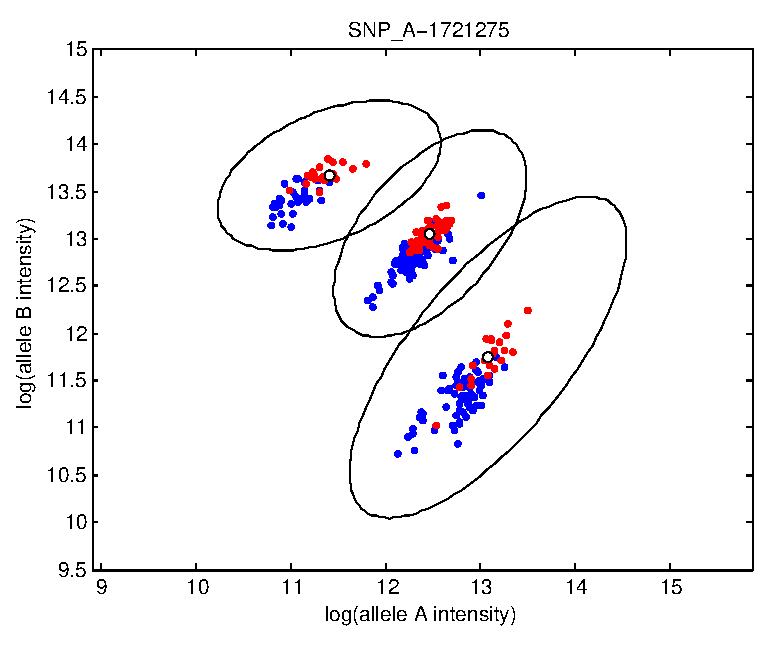
\includegraphics[scale=0.5]
            {result_figs/cmp_socal_gauss_noise_shape/ellipse_no_noise.pdf}
        \label{fig:socal_region_no_noise}
    }
    \subfloat[Decision regions found by RLMM when there is no outlier] {
        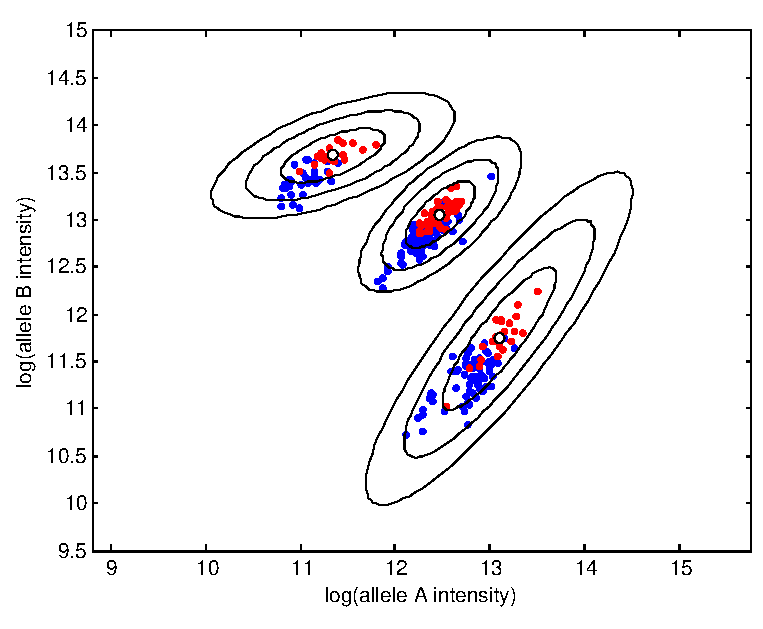
\includegraphics[scale=0.5]
            {result_figs/cmp_socal_gauss_noise_shape/gauss_no_noise.pdf}
        \label{fig:gauss_region_no_noise}
    }
    \\
    \subfloat[Decision regions found by SoCal when there is no outlier] {
        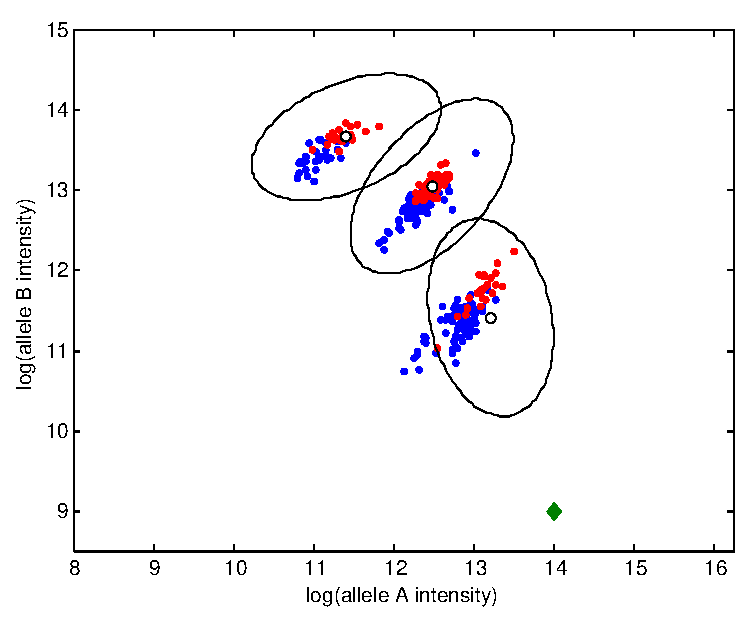
\includegraphics[scale=0.5]
            {result_figs/cmp_socal_gauss_noise_shape/ellipse_noise.pdf}
        \label{fig:socal_region_no_noise}
    }
    \subfloat[Decision regions found by RLMM when there is no outlier] {
        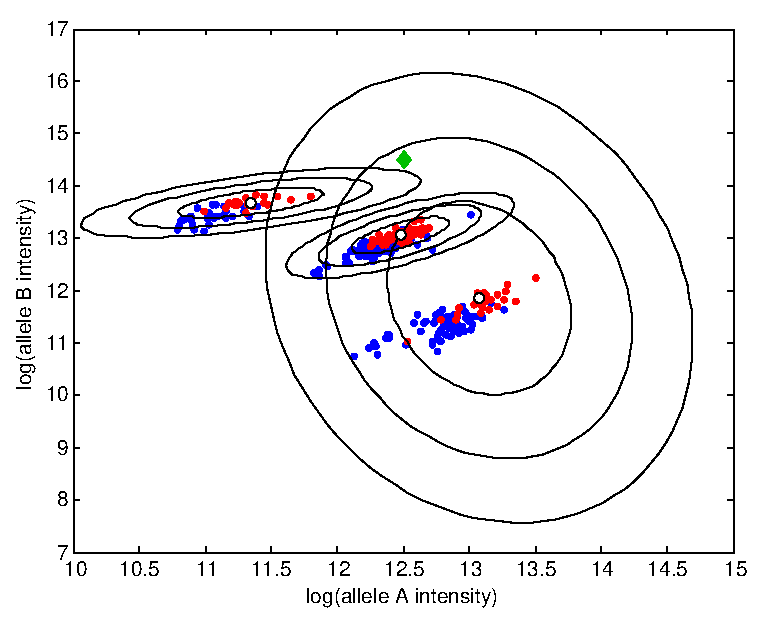
\includegraphics[scale=0.5]
            {result_figs/cmp_socal_gauss_noise_shape/gauss_noise.pdf}
        \label{fig:gauss_region_no_noise}
    }
    \caption{Each dot in the plots above represents a sample, with
             samples having HapMap reference genotype calls marked red.
             The ellipsoids were obtained using only the reference calls.}
    \label{fig:cmp_shape_noise}
\end{figure}

\par
Figure~\ref{fig:result_cmp_noise} shows the decrease in concordance rate of
SoCal and RLMM at call rate of 100\% in leave-one-out cross-validation with
HapMap reference genotype calls as the variance of simulated outliers varies
from 0 to 10.
Clearly, the concordance rate of SoCal decreases much more slowly than does
the RLMM method.
Thus, SoCal is in general more robust to outliers than RLMM.

% accuracy as function of noise variance
\begin{figure}[H]
\centering
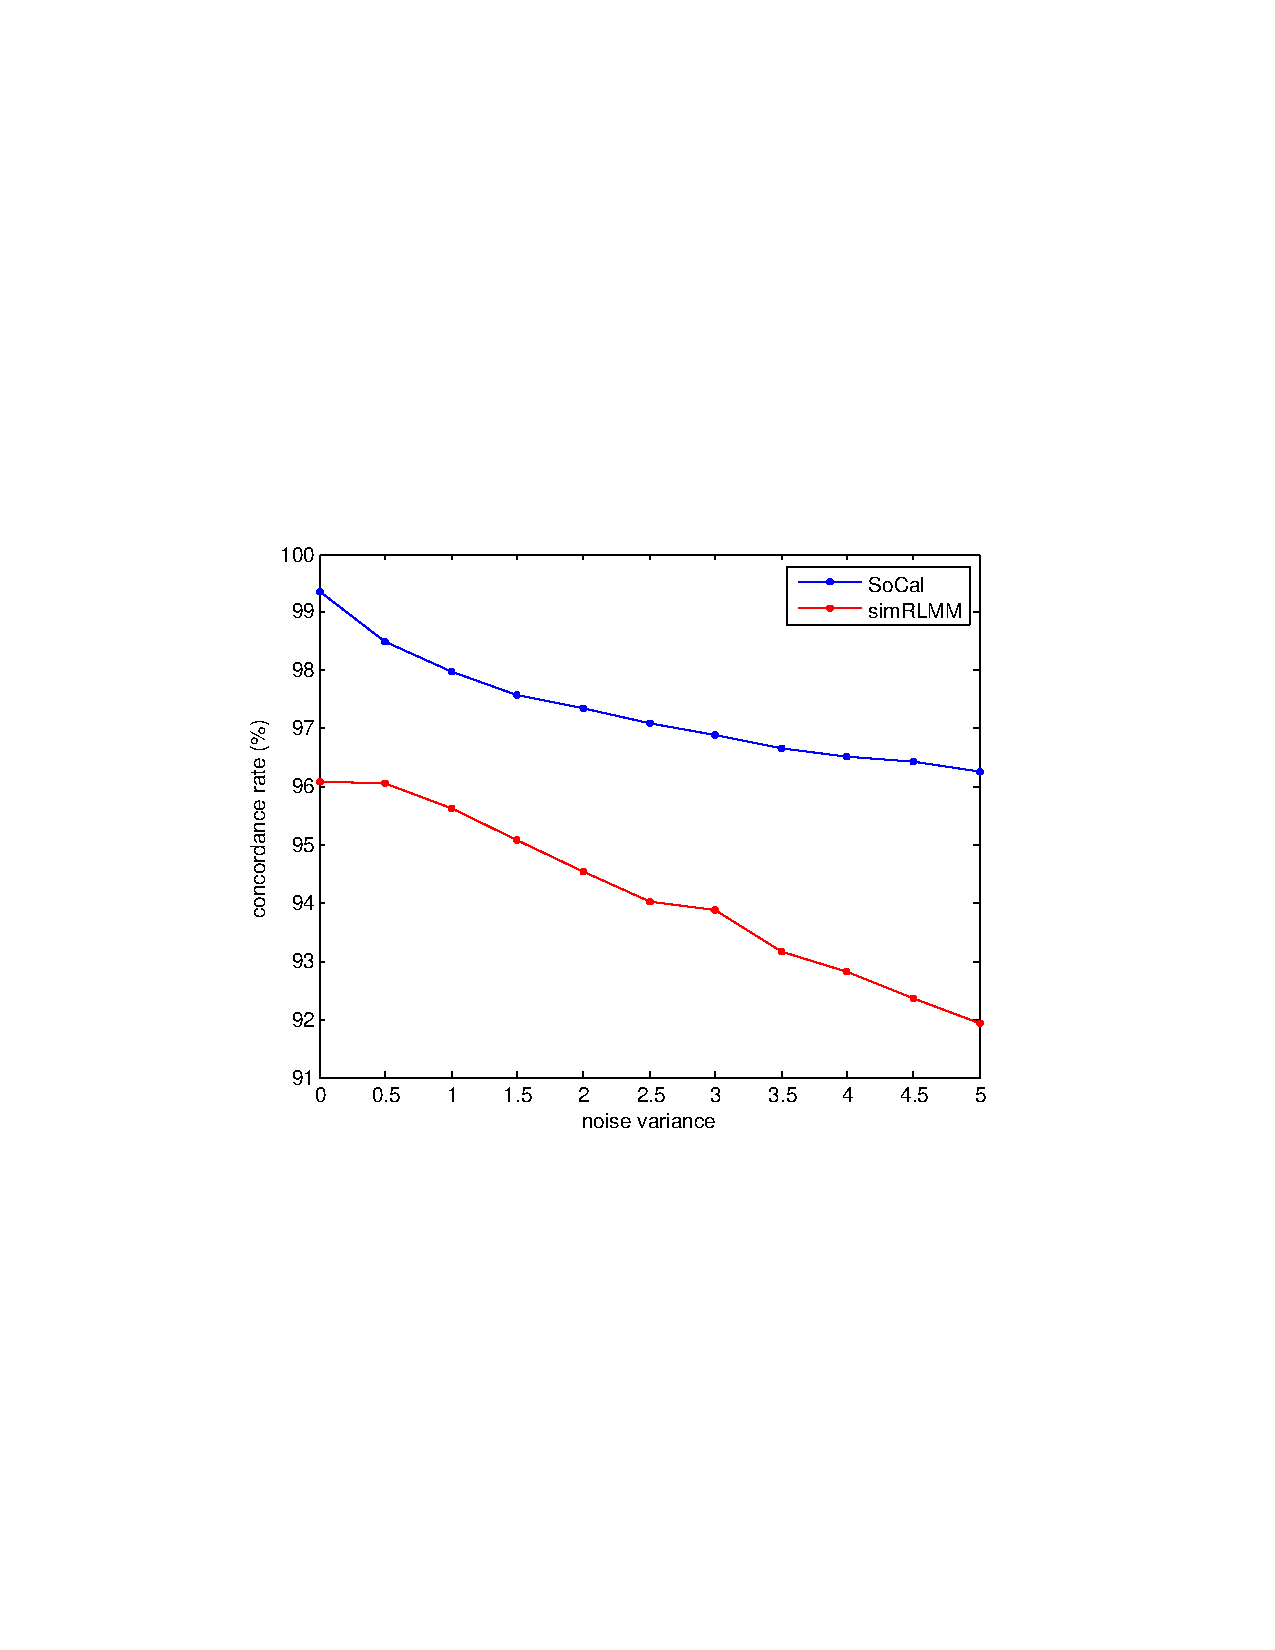
\includegraphics[scale=0.75]
{result_figs/cmp_socal_gauss_noise/socal_gauss_cmp_noise.pdf}
\caption{Concordance rate of SoCal and RLMM in the leave-one-out
cross-validation with HapMap reference calls as a function of outlier
variance.}
\label{fig:result_cmp_noise}
\end{figure}

% implementation
\subsection{Software implementation}
SoCal is implemented in Python.
To solve the conic programming problem of finding separating ellipsoids,
SoCal uses CVXOPT.
Source code of SoCal is available at
\url{https://github.com/huwenboshi/wqe/tree/master/genotype_caller}.
%-----------------------------------------------------------------------------






%-----------------------------------------------------------------------------
% discussion
\section{Discussion}

\par
I have presented SoCal, a supervised genotype calling algorithm for Affymetrix
SNP microarray.
Unlike many existing supervised genotype calling algorithms that try to fit
generative models (mostly Gaussian mixture models) on summarized allele
intensities with reference genotype calls, SoCal uses these data to efficiently
finds ellipsoidal decision regions for each genotype cluster by solving a conic
programming problem.
Both cross-validation of SoCal with HapMap reference calls and comparison with
genotype calls made by CRLMM show that SoCal is comparable in accuracy to many
of the state-of-the-art genotype calling methods.
Also, when there are outliers in training data, SoCal outperforms RLMM, a
genotype calling method that uses Gaussian decision regions to call genotypes,
demonstrating the robustness of SoCal in the presence of outliers over
existing methods.
Overall, SoCal proves to be a promising alternative genotype caller for
Affymetrix SNP microarray.

\par
Like many supervised genotype callers, SoCal has its limitations.
First, SoCal is not directly applicable to SNP microarrays that don't have
reference genotype calls.
Second, SoCal is, in general, also not directly applicable to the same SNP
microarray across different laboratories because different laboratory
protocols can generate different allele intensities for even the same
SNP microarray.
In these scenarios, one can first call genotypes from microarrays using
unsupervised genotype calling algorithms.
One can then use these calls as training data for SoCal and use SoCal to
form refined ellipsoidal decision regions for each genotype cluster.
Because SoCal is robust to outliers in the training data, the refined
ellipsoidal decision regions can be used to accurately call genotypes for
future SNPs.
Another limitation of SoCal is that users need to fine tune the weights
($\beta_i$) assigned to the criteria of finding the ellipsoids.
However, experiments with SoCal show that SoCal is mostly sensitive to the
choice of $\beta_2$ and $\beta_3$.
And optimal values for parameters can be estimated efficiently
through experiments.

\par
SoCal is still in development, and can be improved and extended in
many directions.
First, the current method that SoCal uses to handle SNPs with missing genotype
clusters is through simple and fixed geometric transformations.
This method assumes that genotype AA cluter and genotype BB cluster are
symmetric around genotype AB cluster.
However, this is not true in general.
Future efforts should be spent on how to estimate ellipsoids for missing
genotype clusters more accurately.
Second, currently SoCal only uses allele intensities data for reference
genotype calls.
However, allele intensities data for samples having structual variations is
also available.
A possible improvement for SoCal is to include these data in finding the
ellipsoids for each genotype cluster to further refine the decision regions.
These refined decision regions can then be used to detect possible structural
variations.

\par
To summarize, SoCal presents a novel and promising method for genotype calling.
It's efficient in that it finds decision regions by solving a conic
programming problem, which is solvable in polynomial time with guaranteed
global optimum.
SoCal is also comparable in accuracy with many state-of-the-art methods.
Although SoCal has its limitations, these limitations are also present in other
supervised genotype callers, and have been addressed previously.
SoCal can also be extended and improved to be more accurate and to have more
functionality.
%-----------------------------------------------------------------------------




%-----------------------------------------------------------------------------
% references
\begin{thebibliography}{9}
\bibitem{rho2010}
Rho, S. W., Abell, G. C., Kim, K., Nam, Y., \& Bae, J. (2010).
Comparing microarrays and next-generation sequencing technologies for microbial
ecology research. Trends in Biotechnology, 28, 291-299.
\bibitem{norlen2008}
Norl\'{e}n, H., Pettersson, E., Ahmadian, A., Lundeberg, J., \& Sundberg, R.
(2008). Classification of SNP genotypes by a Gaussian mixture model in
competitive enzymatic assays.
Mathematical Statistics Stockholm University Research Report, 3, 1-26.
\bibitem{lin2008}
Lin, Y., Tseng, G. C., Cheong, S. Y., Bean, L. J., Sherman, S. L., \&
Feingold, E. (2008). Smarter clustering methods for SNP genotype calling.
Bioinformatics, 24, 2665-2671.
\bibitem{wu1983}
Wu, C. F. (1983). On the Convergence Properties of the EM Algorithm.
The Annals of Statistics, 11, 95-103.
\bibitem{rabbee2005}
Rabbee, N., \& Speed, T. P. (2005).
A genotype calling algorithm for affymetrix SNP arrays.
Bioinformatics, 22, 7-12.
\bibitem{zhou2014}
Zhou, X., \& Stephens, M. (2014).
Efficient multivariate linear mixed model algorithms for genome-wide
association studies.
Nature Methods, 11, 407-409.
\bibitem{glineur1998}
Glineur F. (1998). Pattern separation via ellipsoids and conic programming.
(MS Thesis). Faculté Polytechnique de Mons, Mons, Belgium.
\end{thebibliography}
%-----------------------------------------------------------------------------

\end{document}
